\documentclass[aspectratio=169]{beamer}
%\documentclass{beamer}
\usetheme{Madrid}

\usepackage{graphicx}
\usepackage[utf8]{inputenc}
\usepackage{hyperref}
\usepackage{listings}
\usepackage{tikz}
\usetikzlibrary{positioning, arrows.meta, calc, shapes, arrows, positioning}
\usetikzlibrary{}



%\setbeamertemplate{footline}[frame number]

\begin{document}

\title{Introduction to neural networks}  
\subtitle{Recurrent Networks} 
\author[J.I. Vasquez]{\textbf{Juan Irving Vásquez} \\jivg.org}
\date{\today \copyright}
\institute[jivg.org]{Centro de Innovación y Desarrollo Tecnológico en Cómputo \\ Instituto Politécnico Nacional}
\titlegraphic{
\includegraphics[height=1.2cm]{ipn-cidetec.png}\hspace{0.1cm}
\includegraphics[height=1.2cm]{escudoESCOM}}

\frame{\titlepage} 

\frame{
	\frametitle{Contents}
	\tableofcontents
}


\AtBeginSection[] { \begin{frame} \frametitle{Roadmap} \tableofcontents[currentsection] \end{frame} }


\section{Motivation}


\begin{frame}
	\frametitle{Motivation}
	\begin{columns}
	\column{0.5\textwidth}
	\textbf{Sequential Data}
	\begin{itemize}
		\item Order matters. Current output depends on history.
		\item Examples:
		\begin{itemize}
			\item \textbf{Time Series:} Stock prices, weather data.
			\item \textbf{NLP:} Translation, Sentiment Analysis.
			\item \textbf{Audio:} Speech recognition.
		\end{itemize}
	\end{itemize}
	
	\column{0.5\textwidth}
		\begin{figure}
			\centering
			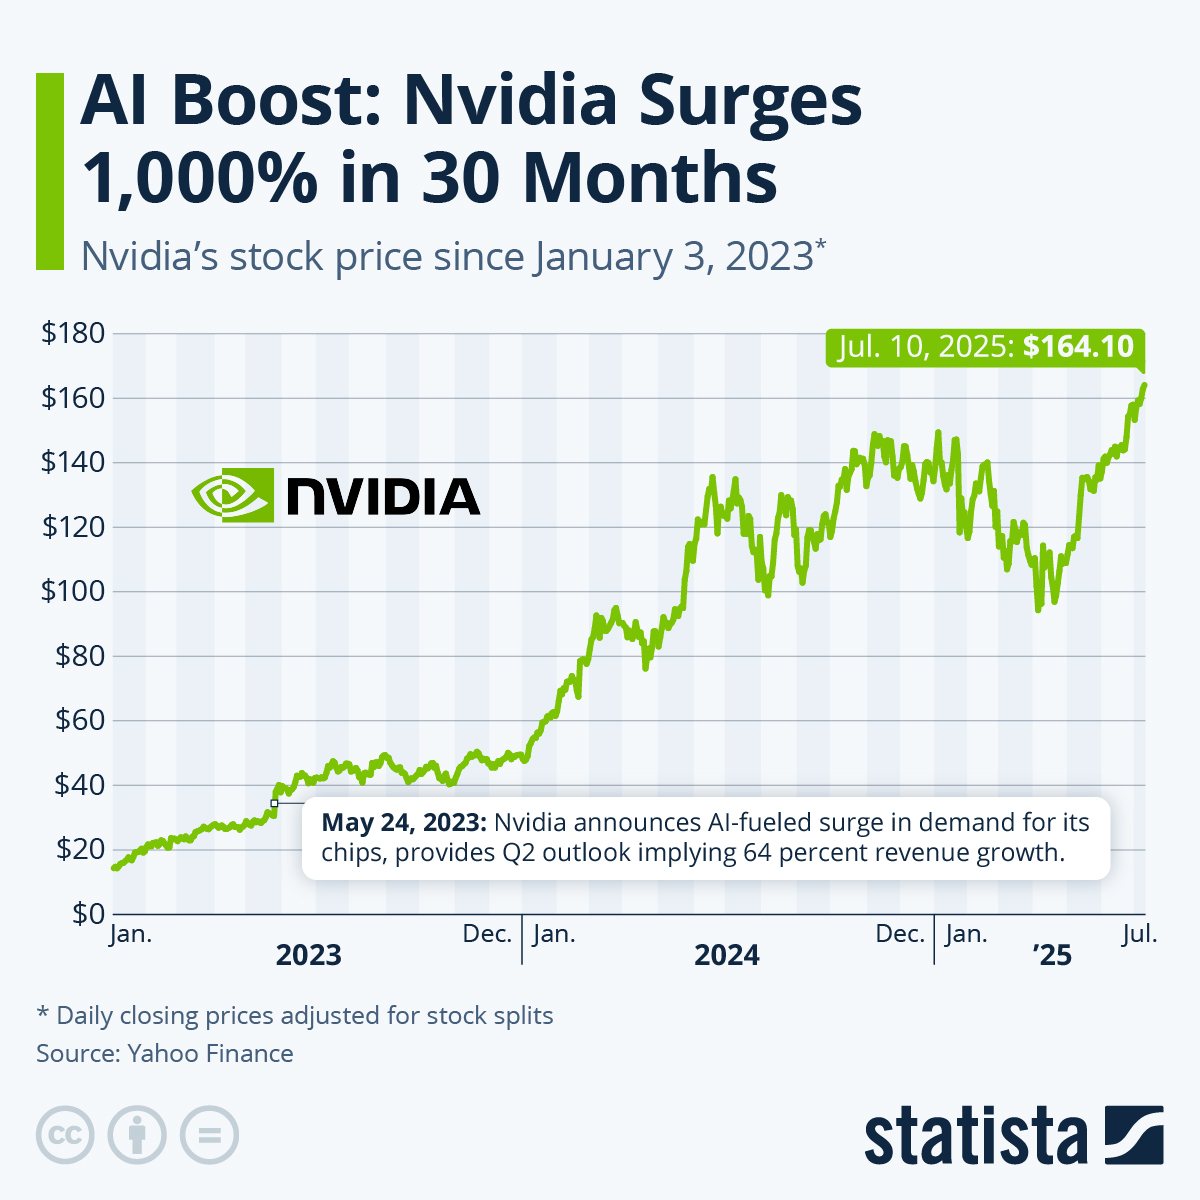
\includegraphics[height=0.65\textheight]{32358}
			\caption{Nvidia Stock prices \footnote{\scriptsize https://www.statista.com/}}
			\label{fig:32358}
		\end{figure}
\end{columns}
\end{frame}



\begin{frame}{Motivation}
	\framesubtitle{Usinng feed forward networks in sequential data}
	\begin{columns}
		\column{0.5\textwidth}
		\begin{itemize}
		\item Feed forward networks (FFN), e.g. the multilayer perceptrion, have fixed input size.
		\item Nevertheless, they can be used as follows:
		\begin{itemize}
			\item Size larger than input (the inpunt is filled)
			\item Size equals input (ralerly occurs)
			\item Size is shorter than input (only a section is analyzed)
		\end{itemize}
	   \end{itemize}
		\column{0.5\textwidth}
		\begin{figure}
			\centering
			
\includegraphics[height=0.7\textheight]{input}
			\caption{Different size inputs problem.}
			\label{fig:input}
		\end{figure}
	\end{columns}
\end{frame}


\begin{frame}
	\frametitle{Seq2seq with Neural N-Grams}
	\framesubtitle{Example of using FFN in sequences}
\begin{center}
	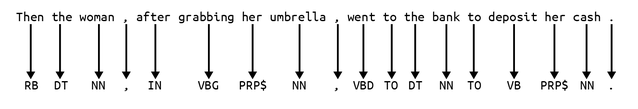
\includegraphics[height=0.25\textheight]{seq2seq}
\end{center}

\begin{center}
	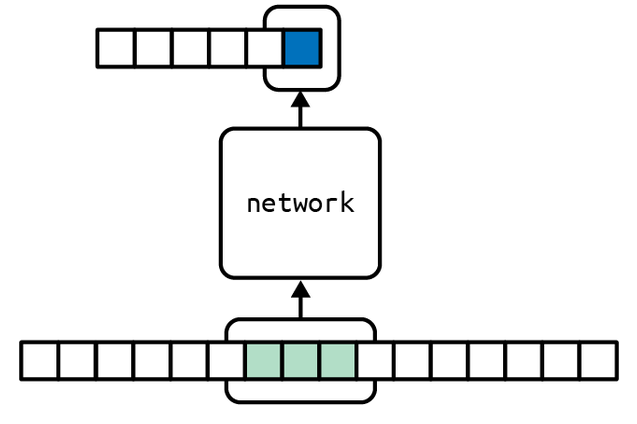
\includegraphics[height=0.5\textheight]{ngram}
\end{center}
\end{frame}

\begin{frame}{Feedforward vs. Recurrent}
	\begin{columns}
		\column{0.5\textwidth}
		\begin{itemize}
			\item Feedforward Neural Network (FNN)
			\begin{itemize}
				\item Information flows in one direction: \\ Input $\rightarrow$ Hidden $\rightarrow$ Output.
			\end{itemize}
		\end{itemize}
		
		\vspace{0.5cm}
		
		\begin{itemize}
			\item Recurrent Neural Network (RNN). \\ Contains a \textbf{loop}. The output of a neuron is fed back into itself as input for the next time step.
			\begin{itemize}
				\item Maintains an internal state (memory).
				\item Uses \textbf{Shared Weights} across all time steps.
			\end{itemize}
		\end{itemize}
		
		\column{0.5\textwidth}
		
		\begin{figure}
			\centering
			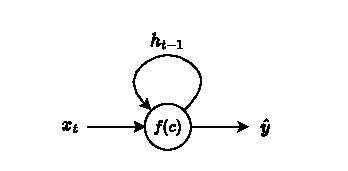
\includegraphics[width=\linewidth]{recurrent_nn.drawio}
			\caption{Simple recurrent neural node}
			\label{fig:recurrentnn}
		\end{figure}
\end{columns}
	
	
	
\end{frame}


\section{Recurrent network}


\begin{frame}{Recurrent neural network}
	At time step $t$, the hidden state $h_t$ is updated using the input $x_t$ and the previous hidden state $h_{t-1}$.	
	\begin{equation}
		\mathbf{h}_t = f(W_h \mathbf{h}_{t-1} + W_x X_t + b)
	\end{equation}
	where:
	\begin{itemize}
		\item $\mathbf{h}_t$: New hidden state.
		\item $\mathbf{h}_{t-1}$: Old hidden state (memory from previous step).
		\item $X_t$: Current input vector.
		\item $W_h, W_x$: Weight matrices (Trainable parameters).
		\item $f(c)$: Activation function.
	\end{itemize}
\end{frame}


\begin{frame}{Recurrent neural network}
	The predicion is based on the hidden state.
	\begin{itemize}
		\item For simplicity:
		\begin{equation}
			\hat{y} = \mathbf{h}_T
		\end{equation} where $T$ is the lenght of the input.
		\item in general:
				\begin{equation}
			\hat{y} = \mathbf{h}_T W_y
		\end{equation} where $W_y$ is a trainable matrix.
	\end{itemize}
\end{frame}



\begin{frame}{Unrolling through time}
	To understand RNNs, we visualize them as multiple copies of the same network, each passing a message to a successor.
	
	\vspace{1cm}
	
	\centering
	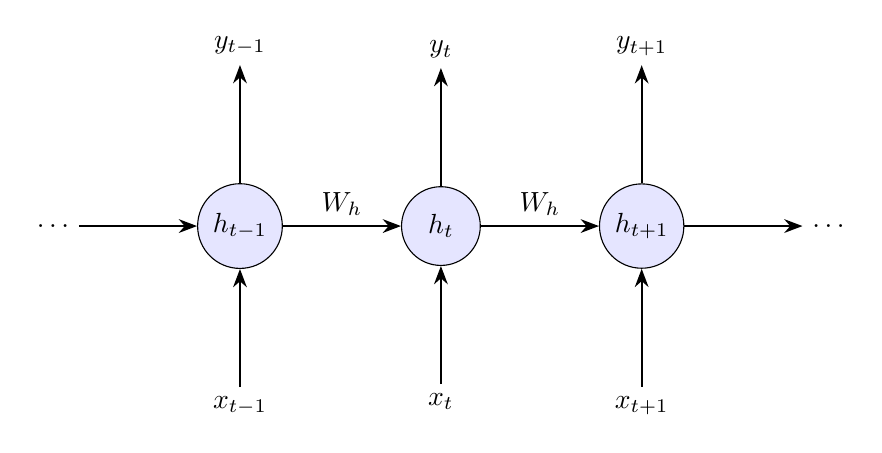
\begin{tikzpicture}[
		node distance=1.5cm,
		layer/.style={circle, draw, minimum size=1cm, fill=blue!10},
		arrow/.style={-Stealth, thick}
		]
		% Time step t-1
		\node[layer] (h_prev) {$h_{t-1}$};
		\node[below=of h_prev] (x_prev) {$x_{t-1}$};
		\node[above=of h_prev] (y_prev) {$y_{t-1}$};
		
		% Time step t
		\node[layer, right=of h_prev] (h_curr) {$h_t$};
		\node[below=of h_curr] (x_curr) {$x_t$};
		\node[above=of h_curr] (y_curr) {$y_t$};
		
		% Time step t+1
		\node[layer, right=of h_curr] (h_next) {$h_{t+1}$};
		\node[below=of h_next] (x_next) {$x_{t+1}$};
		\node[above=of h_next] (y_next) {$y_{t+1}$};
		
		% Connections
		\draw[arrow] (x_prev) -- (h_prev);
		\draw[arrow] (h_prev) -- (y_prev);
		
		\draw[arrow] (x_curr) -- (h_curr);
		\draw[arrow] (h_curr) -- (y_curr);
		
		\draw[arrow] (x_next) -- (h_next);
		\draw[arrow] (h_next) -- (y_next);
		
		% Recurrent connections
		\draw[arrow] (h_prev) -- node[above] {$W_h$} (h_curr);
		\draw[arrow] (h_curr) -- node[above] {$W_h$} (h_next);
		
		% Ellipsis
		\node[left=of h_prev] (start) {$\dots$};
		\draw[arrow] (start) -- (h_prev);
		\node[right=of h_next] (end) {$\dots$};
		\draw[arrow] (h_next) -- (end);
		
	\end{tikzpicture}
\end{frame}


% =========================================================================
\section{Training \& Challenges}
% =========================================================================

\begin{frame}{Backpropagation Through Time (BPTT)}
	\begin{itemize}
		\item Training is similar to standard Backpropagation, but gradients flow backward through time.
		\item We compare the predicted sequence to the target sequence to compute Loss ($L$).
		\item We compute $\frac{\partial L}{\partial W}$ by summing gradients at each time step.
	\end{itemize}

\end{frame}


\frame{
	\frametitle{Backprogation implementation}
	\begin{itemize}
		\item In the output layer you have error at time $T$ (last time),
		\item We can generalize previous error term as $\delta_t$,
		\item Term error for hidden layer node $t$,
		\begin{equation}
			\delta_t = w_{h} \delta_{t+1} f'(c_t),
		\end{equation} where $c$ is the linear combination 
		\item The increment is computed by time, 
		\begin{equation}
			\Delta w_{x|t} = \eta \delta_t x_{i}
		\end{equation}
		\begin{equation}
			\Delta w_{h|t} = \eta \delta_t h_{i}
		\end{equation}
		\begin{equation}
			\Delta b{t} = \eta \delta_t (1)
		\end{equation}
	\end{itemize}
}



\begin{frame}{The Vanishing Gradient Problem}
		\textbf{The Problem:}
	\begin{itemize}
		\item Since the same matrix $W$ is multiplied repeatedly (chain rule) during backpropagation...
		\item If weights are small ($<1$), gradients shrink exponentially $\rightarrow$ \textbf{Vanishing Gradient}.
		\item If weights are large ($>1$), gradients grow exponentially $\rightarrow$ \textbf{Exploding Gradient}.
	\end{itemize}
	\begin{alertblock}{Consequence}
		The network effectively stops learning from early inputs in long sequences. \\ It suffers from \textbf{Short-Term Memory}.
	\end{alertblock}
	\textbf{Example:}
	\begin{quote}
		"I grew up in \textbf{France}... [long paragraph] ... I speak fluent \textbf{French}."
	\end{quote}
	
	An RNN with vanishing gradients might forget the context "France" by the time it needs to predict "French".
\end{frame}

% =========================================================================
\section{Extensions: LSTM and GRU}
% =========================================================================

\begin{frame}{Solution: Long Short-Term Memory (LSTM)}
	Introduced by Hochreiter \& Schmidhuber en 1997\footnote{\scriptsize Hochreiter, S., \& Schmidhuber, J. (1997). Long short-term memory. Neural computation, 9(8), 1735-1780.}.
	\begin{columns}
		\column{0.5\textwidth}
		\begin{itemize}
			\item Introduces a \textbf{Cell State} ($C_t$) acting as an information highway.
			\item Uses \textbf{Gates} to regulate information flow:
			\begin{enumerate}
				\item \textbf{Forget Gate:} What to remove from memory?
				\item \textbf{Input Gate:} What new info to store?
				\item \textbf{Output Gate:} What to show as output?
			\end{enumerate}
		\end{itemize}
		\column{0.5\textwidth}
\begin{figure}
	\centering
	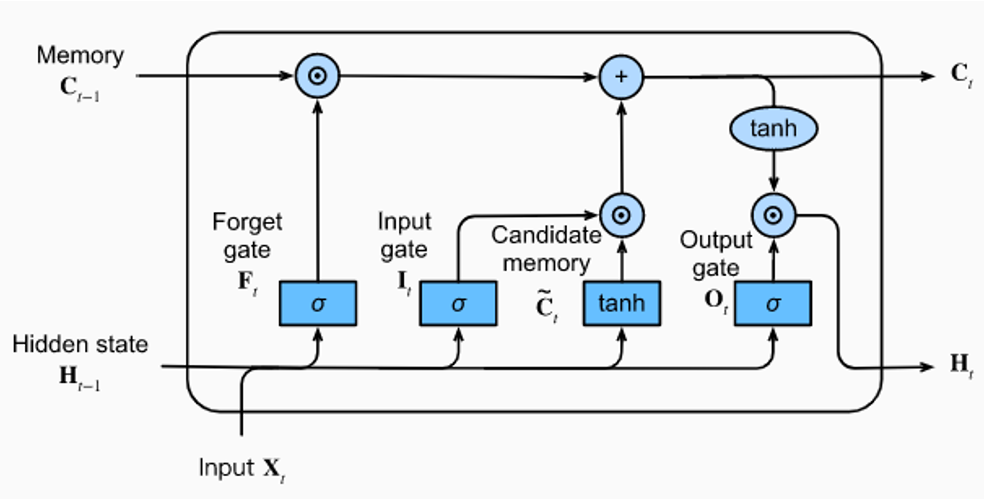
\includegraphics[width=\linewidth]{1_Mb_L_slY9rjMr8-IADHvwg}
	\caption{LSTM neural network}
	\label{fig:1mblsly9rjmr8-iadhvwg}
\end{figure}
	\end{columns}
\end{frame}


\begin{frame}{LSTM (Cell state)}
	Cell state computation:
	\begin{equation}
		C_t = f_t \odot C_{t-1} + i_t \odot \tilde{C}_t
	\end{equation}
	where,
	\begin{itemize}
		\item  $f_t$: forget gate. How much of the past cell state should be forgotten,
		$$f_t = \sigma(W_{fx} x_t + W_{fh} h_{t-1} + b_f)$$	
		\item $i_t$: The input gate. It decides which new information from the current input will be allowed to update the cell state,
		$$i_t = \sigma(W_{ix} x_t + W_{ih} h_{t-1} + b_i)$$ 
		\item $\tilde{C}_t$: The candidate cell state,
		$$\tilde{C}_t = \tanh(W_{cx} x_t + W_{ch} h_{t-1} + b_c)$$
		\item $\odot$: Hadamard product (element-wise multiplication).
	\end{itemize}
\end{frame}


\begin{frame}{LSTM (Hidden state)}
	Hidden state computation:
	\begin{equation}
		h_t = o_t \odot \tanh(C_t)
	\end{equation}
	where $o_t$ is the output gate:
	\begin{equation}
		o_t = \sigma(W_{ox} x_t + W_{oh} h_{t-1} + b_o)
	\end{equation}
\end{frame}



\begin{frame}{Alternative: Gated Recurrent Unit (GRU)}
	Introduced by Cho et al., en 2014\footnote{\scriptsize Cho, K., Van Merriënboer, B., Gulcehre, C., Bahdanau, D., Bougares, F., Schwenk, H. and Bengio, Y., 2014. Learning phrase representations using RNN encoder-decoder for statistical machine translation. arXiv preprint arXiv:1406.1078.}.
	\begin{columns}
    	 \column{0.5\textwidth}
	 	 \begin{itemize}
		 	\item A simplified version of LSTM.
		 	\item Merges the Cell State and Hidden State.
		 	\item Combines Forget and Input gates into a single \textbf{Update Gate}.
		 	\item \textbf{Benefit:} Fewer parameters, faster to train, often performs just as well.
		 \end{itemize}
	 
		 \column{0.5\textwidth}		 
		\begin{figure}
			\centering
			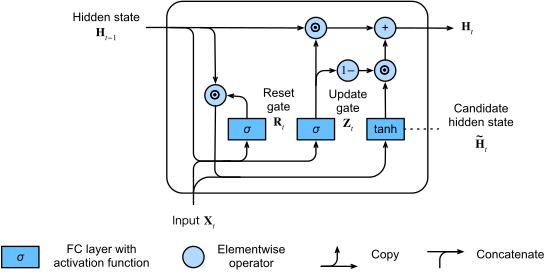
\includegraphics[width=\linewidth]{gru-3}
			\caption{GRU neural network}
			\label{fig:gru-3}
		\end{figure}
	\end{columns}
\end{frame}


\section{Application to NLP}



\begin{frame}{Introduction to NLP}
	\begin{block}{A functional definition}
		Using machine learning and large datasets to give computers the ability \textbf{NOT} to understand language, but to ingest a piece of language as input and return something useful.
	\end{block}
	
	\textbf{Predicting the useful output:}
	\begin{itemize}
		\item \textit{``What’s the topic of this text?''}  $\rightarrow$ \textbf{Text classification}
		\item \textit{``Does this text contain abuse?''}  $\rightarrow$ \textbf{Content filtering}
		\item \textit{``Does this text sound positive or negative?''}  $\rightarrow$ \textbf{Sentiment analysis}
		\item \textit{``What should be the next word in this incomplete sentence?''}  $\rightarrow$ \textbf{Language modeling}
		\item \textit{``How would you say this in German?''}  $\rightarrow$ \textbf{Translation}
		\item \textit{``How would you summarize this article in one paragraph?''}  $\rightarrow$ \textbf{Summarization}
	\end{itemize}
\end{frame}

%\subsection{Encoder-Decoder Architecture}

%\subsection{Sequence-to-Sequence (Seq2Seq)}


% --- Slide: Text Processing Models ---
\begin{frame}{Text Processing Models}
	There are two main kinds of text-processing models:
	\vspace{0.5cm}
	\begin{itemize}
		\item \textbf{Sequence models:} Care about word order. They use word-level tokenization.
		\item \textbf{Bag-of-words models:} Treat input words as a set, discarding their original order. They use N-gram tokenization.
	\end{itemize}
\end{frame}

\begin{frame}{Sequence-to-Sequence (Seq2Seq) tasks}
	\begin{itemize}
		\item Are tasks where the inputs and outputs are sequences.
		\item Example (Machine translation):
		\begin{itemize}
			\item Input: \textit{J'aime le thé.} (French)
			\item Output: \textit{I love tea.} (English)
		\end{itemize}
		\item \textbf{Special Tokens:} They are additional to the sentence.
		\begin{itemize}
			\item \texttt{<bos>}: Beginning of sentence.
			\item \texttt{<eos>}: End of sentence.
		\end{itemize}
		%\item \textbf{Connection:} The final hidden state of the encoder acts as the initial input for the decoder.
	\end{itemize}
\end{frame}

%

% --- Slide: Preparing text data (Two Columns) ---
\begin{frame}{Data preprocessing}
\framesubtitle{Vectorization}
	\begin{columns}[T] % T aligns the content at the top
		% First Column: Definitions
		\begin{column}{0.48\textwidth}
			\begin{itemize}
				\item Deep learning models are differentiable functions that can only process numeric tensors: \textbf{they cannot take raw text as input}.
				\vspace{0.5cm}
				\item \textbf{Vectorization:} The process of transforming text into numeric tensors.
			\end{itemize}
		\end{column}
		
		% Second Column: Example Process
		\begin{column}{0.48\textwidth}
			\small
			Original Text: ("The cat sat on the mat.")
			\begin{enumerate}
				\item \textbf{Standardization:} \\ ("the cat sat on the mat")
				\item \textbf{Tokenization:} \\ ("the", "cat", "sat", "on", "the", "mat")
				\item \textbf{Indexing:} \\ (3, 26, 65, 9, 3, 133)
				\item \textbf{One-hot encoding:} \\ (Vector Representation).
			\end{enumerate}
		\end{column}
	\end{columns}
\end{frame}


% --- Slide: Tokenization ---
\begin{frame}{Tokenization}
	\begin{columns}
		\begin{column}{0.5\textwidth}
				There are different strategies for splitting text:
			\begin{itemize}
				\item \textbf{Word-level tokenization:} Tokens are space-separated (or punctuation-separated) substrings.
				\item \textbf{N-gram tokenization:} Tokens are groups of $N$ consecutive words (e.g., "the cat" is a 2-gram or bigram).
				\item \textbf{Character-level tokenization:} Each character is its own token.
			\end{itemize}
		\end{column}
	
		\begin{column}{0.5\textwidth}
\begin{center}
	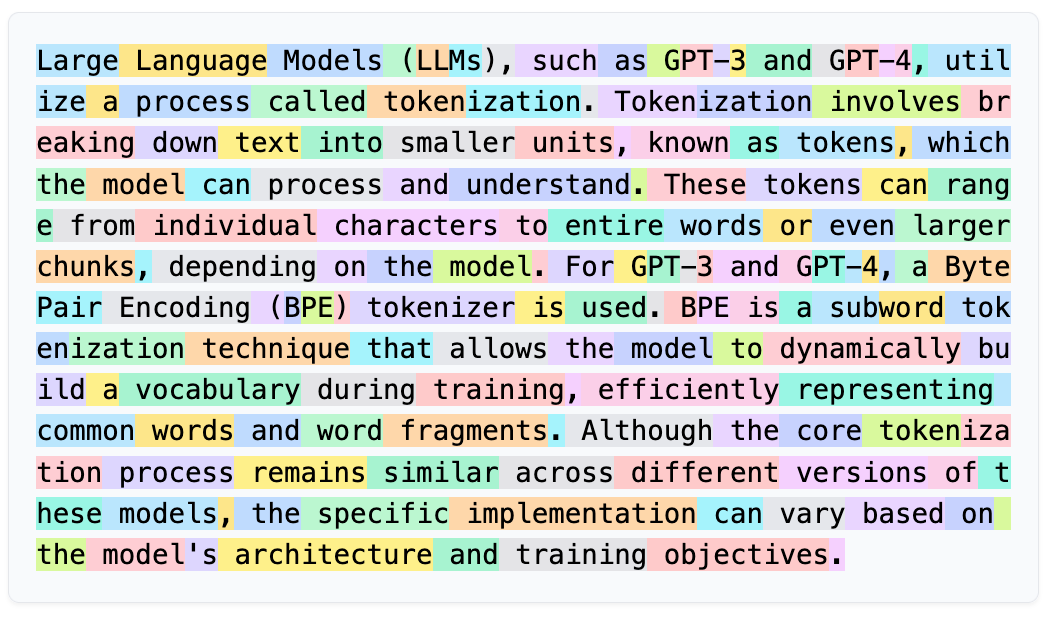
\includegraphics[width=0.9\linewidth]{../19_transformers/tokenization}
\end{center}
		\end{column}
	\end{columns}
\end{frame}


\begin{frame}{N-grams}
	\begin{block}{Definition}
		Word N-grams are groups of $N$ (or fewer) consecutive words that can be extracted from a sentence.
	\end{block}
	
	\textbf{Example:} "the cat sat on the mat."
	\begin{itemize}
		\item \textbf{Set of 2-grams:} \{"the", "the cat", "cat", "cat sat", "sat", "sat on", "on", "on the", "the mat", "mat"\}.
		\item \textbf{Set of 3-grams:} \{"the", "the cat", "cat", "cat sat", "the cat sat", "sat", ...\}.
	\end{itemize}
\end{frame}

% --- Slide: Vocabulary indexing ---
\begin{frame}[fragile]{Vocabulary Indexing}
	\begin{itemize}
		\item Once text is split into tokens, they must be encoded numerically. 
		\item In practice, an index of all terms in the training data (the "vocabulary") is built, and a unique integer is assigned to each entry.
	\end{itemize}
\begin{figure}
	\centering
	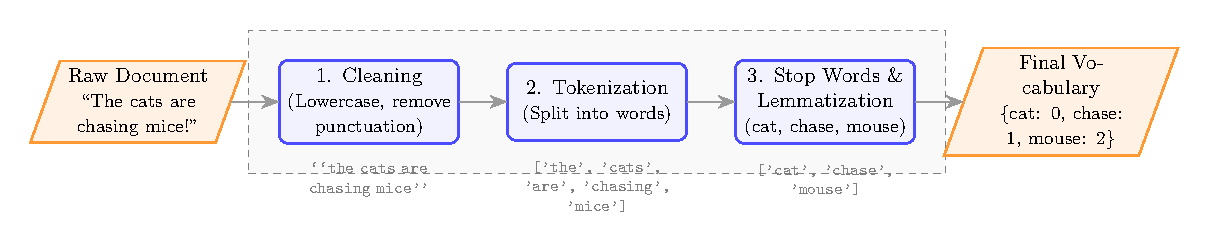
\includegraphics[width=0.9\linewidth]{figura_vocabulary}
	\caption{Vocabulary creation}
	\label{fig:figuravocabulary}
\end{figure}
\end{frame}


\begin{frame}{Encoder-decoder architecture}
	\begin{itemize}
		\item \textbf{Problem Domain:} Seq2seq problems.
		\item \textbf{Variable Lengths:} Generally, input and output sequences have different lengths.
		\item \textbf{The architecture} for this problem:
		\begin{itemize}
			\item \textbf{Encoder:} Converts a variable-length sequence into a \textit{fixed-length} output state.
			\item \textbf{Context state:} Acts as a bottleneck or compressed representation.
			\item \textbf{Decoder:} Converts the fixed-length state back into a variable-length output.
		\end{itemize}
	\end{itemize}
	
	\vspace{0.5cm}
	
	% Simple TikZ diagram for the abstract architecture
	\centering
	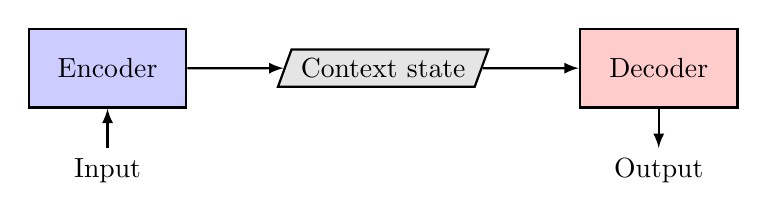
\begin{tikzpicture}[node distance=2cm, auto, >=latex, thick]
		\node [draw, rectangle, fill=blue!20, minimum height=1cm, minimum width=2cm] (enc) {Encoder};
		\node [draw, trapezium, trapezium left angle=70, trapezium right angle=110, fill=gray!20, right of=enc, node distance=3.5cm] (state) {Context state};
		\node [draw, rectangle, fill=red!20, minimum height=1cm, minimum width=2cm, right of=state, node distance=3.5cm] (dec) {Decoder};
		
		\draw [->] (enc) -- (state);
		\draw [->] (state) -- (dec);
		\draw [<-] (enc.south) -- ++(0,-0.5) node[below] {Input};
		\draw [->] (dec.south) -- ++(0,-0.5) node[below] {Output};
	\end{tikzpicture}
\end{frame}


\begin{frame}{The Encoder: Mathematical Formulation}
	\begin{itemize}
		\item 	The input sequence is represented as vectors, $x_1, \dots, x_T$, (after tokenization and embedding).
		\begin{equation}
			X = \begin{bmatrix}
				\begin{bmatrix} x_{1,1} & x_{1,2} & \dots & x_{1,d} \end{bmatrix} \\				\vdots \\
				\begin{bmatrix} x_{n,1} & x_{n,2} & \dots & x_{n,d} \end{bmatrix}
			\end{bmatrix}
		\end{equation}
		\item A RNN generates a new hidden state $h_t$ based on the previous state $h_{t-1}$ and current input $x_t$:
		\begin{equation}
			\mathbf{h}_t = f(\mathbf{h}_{t-1}, x_t)
		\end{equation}
		Concretely (using tanh activation):
		\begin{equation}
			\mathbf{h}_t = \tanh(W_{h}\mathbf{h}_{t-1} + W_{x}x_t + b)
		\end{equation}
	\end{itemize}
\end{frame}


\begin{frame}{The Context Vector}
	\begin{itemize}
		\item The \textbf{Context Variable (or Vector)} $c$ must encode the information of the \textit{entire} input sequence.
		\item It is defined by a mapping function $m$:
		\begin{equation}
			c = m(\mathbf{h}_1, \dots, \mathbf{h}_T)
		\end{equation}
		\item In the simplest case, it is just the last hidden state of the encoder:
		\begin{equation}
			c = \mathbf{h}_T
		\end{equation}
		%\item \textbf{Bidirectional RNNs:} The state may depend on both previous ($h_{t-1}$) and future ($h_{t+1}$) states.
	\end{itemize}
\end{frame}

\begin{frame}{The Decoder}
	\begin{itemize}
		\item The decoder generates the output sequence $\hat{y}_1, \dots, \hat{y}_{T'}$.
		\item Inputs to decoder:
		\begin{enumerate}
			\item Context variable: $c$
			\item Previous output token: $\hat{y}_{t'-1}$
			\item Previous decoder hidden state: $s_{t'-1}$
		\end{enumerate}
		\item Decoder state update
	\begin{equation}
	s_{t'} = g(s_{t'-1}, \hat{y}_{t'-1}, c)
\end{equation}
	\end{itemize}
		
	\begin{block}{Output Probability}
		The conditional distribution of the next token is calculated via Softmax:
		\begin{equation}
			P(\hat{y}_{t'} | \hat{y}_{t'-1}, \dots, \hat{y}_1, c) = \text{SoftMax}(s_{t'})
		\end{equation}
	\end{block}
\end{frame}

\begin{frame}{Training the Seq2Seq Model}
	\begin{itemize}
		\item \textbf{Joint Training:} The encoder and decoder are trained together.
		\item \textbf{Loss Function:} Cross-entropy loss is used for optimization:
		\begin{equation}
			\max_{\theta} \frac{1}{N} \sum_{n=1}^{N} \log p_{\theta}(\hat{y}^{(n)} | x^{(n)})
		\end{equation}
		\item \textbf{Teacher Forcing:}
		\begin{itemize}
			\item A technique to address slow convergence and instability.
			\item The ground truth (original output sequence) is used as input to the decoder during training, rather than the model's own previous prediction.
		\end{itemize}
	\end{itemize}
\end{frame}


\frame{
	\frametitle{Great advances!}
	\begin{itemize}
		\item FCN, CNN, RNN, ResNet were having great succeful
		\begin{figure}
			\centering
			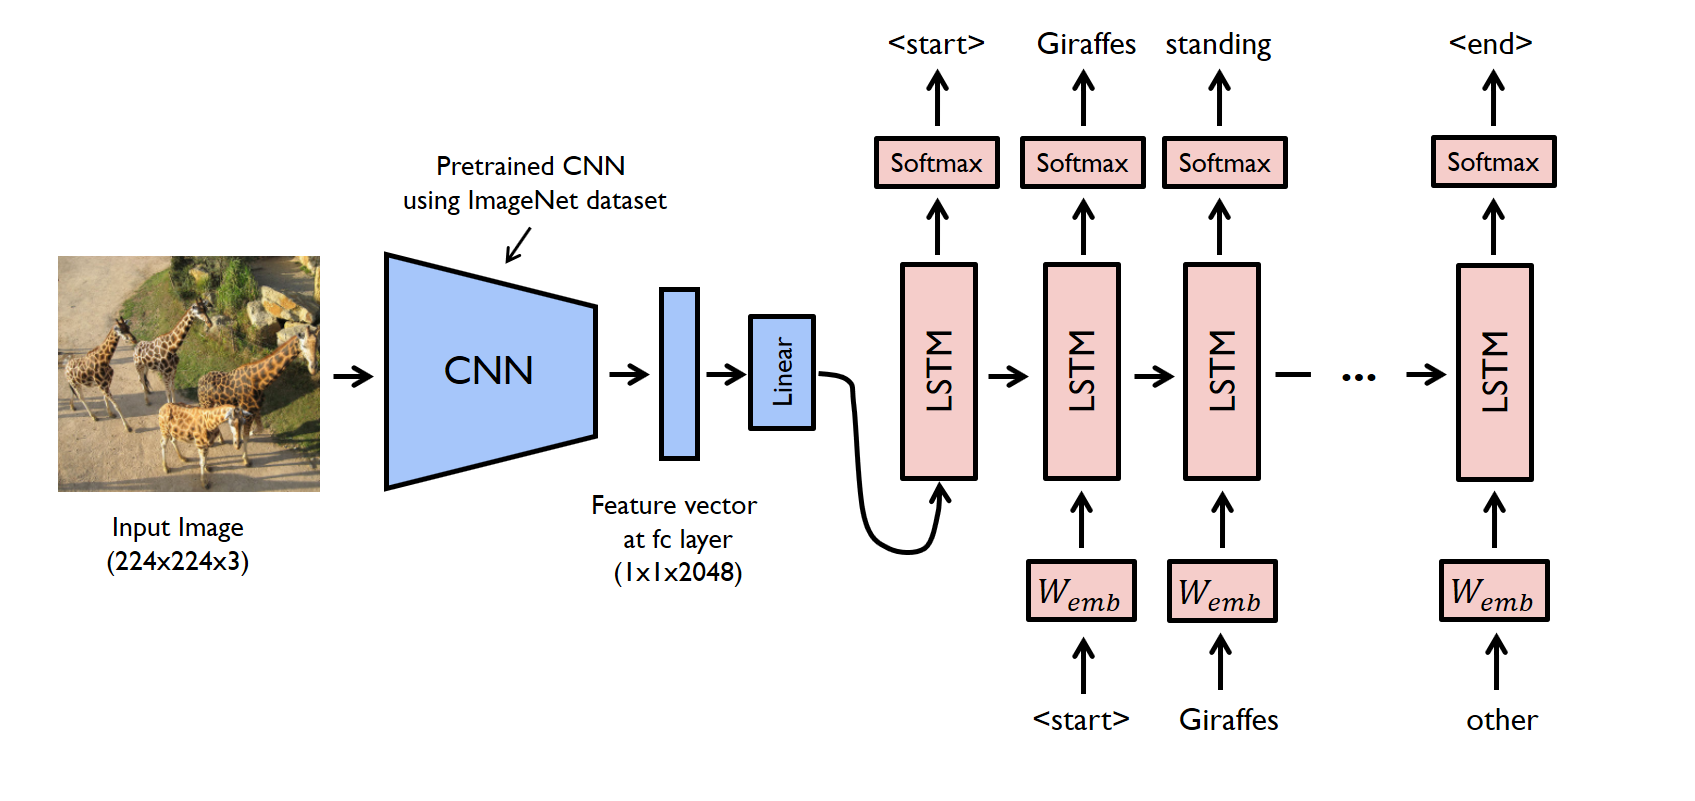
\includegraphics[width=0.75\linewidth]{model}
			%\caption{}
			\label{fig:model}
		\end{figure}	
		\item But they were limited by the supervised approach
		\item RNN struggled to parse longer chunks of text
	\end{itemize}
}


% =========================================================================
%\section{Conclusion}
% =========================================================================

\begin{frame}{Summary}
	\begin{itemize}
		\item \textbf{RNNs} are designed for sequential data where history matters.
		\item They share weights across time steps ($W_h, W_x$).
		\item Training is done via \textbf{Backpropagation Through Time (BPTT)}.
		\item \textbf{Vanishing Gradients} make standard RNNs hard to train on long sequences.
		\item \textbf{LSTMs and GRUs} decrease this using gating mechanisms to preserve long-term dependencies.
	\end{itemize}
\end{frame}


\begin{frame}
	\frametitle{References}
	\begin{itemize}
		\item Du, K.L. and Swamy, M.N., 2013. Neural networks and statistical learning. Springer Science \& Business Media.
		\item Zhang, A., Lipton, Z.C., Li, M. and Smola, A.J., 2023. Dive into deep learning. Cambridge University Press.
		\item Goodfellow, Ian, Yoshua Bengio, and Aaron Courville. Deep learning. MIT press, 2016.
		\item NYU, Aprendizaje profundo,  \url{https://atcold.github.io/pytorch-Deep-Learning/es/week07/07-3/} 
	\end{itemize}
\end{frame}


\end{document}

